\documentclass[conference]{IEEEtran}
\IEEEoverridecommandlockouts
\usepackage{cite}
\usepackage{amsmath,amssymb,amsfonts}
\usepackage{algorithmic}
\usepackage{graphicx}
\usepackage{textcomp}
\usepackage{xcolor}
\usepackage{booktabs}
\usepackage{multirow}
\usepackage{url}
\def\BibTeX{{\rm B\kern-.05em{\sc i\kern-.025em b}\kern-.08em
    T\kern-.1667em\lower.7ex\hbox{E}\kern-.125emX}}

\begin{document}

\title{Fair-RLVR: Reducing Stereotype Bias in LLM Reasoning via Verifiable Benchmark Rewards}

\author{\IEEEauthorblockN{
Salo Edwin Soja\textsuperscript{*},
Arjun Geetha Ravi\textsuperscript{\ddag},
Devanand Asokan\textsuperscript{\dag}, and
Rini Susan Vjayakumar Senla\textsuperscript{\S}}
\IEEEauthorblockA{\textsuperscript{*}Infosys \quad
\textsuperscript{\ddag}Independent Researcher \quad
\textsuperscript{\dag}IBM \quad
\textsuperscript{\S}Santa Clara University, CA, USA}
\IEEEauthorblockA{Emails: \{salosoja, arjungravi1, a.devanand007\}@gmail.com, rvijayakumarsenlakum@scu.edu}
}

\maketitle

\begin{abstract}
Current methods for reducing bias in large language models, such as Reinforcement Learning from Human Feedback (RLHF), rely on subjective human judgments that are inconsistent, expensive, and prone to teaching surface-level compliance rather than principled stereotype avoidance. While recent work has shown that verifiable rewards can teach models to reason through complex tasks like mathematics, no prior work has applied this approach to fairness, despite bias benchmarks providing clear ground-truth labels.

This paper introduces Fair-RLVR, a framework that uses the Bias Benchmark for Question Answering (BBQ) whose ambiguous-context questions have objectively verifiable labels as an automated reward signal for Group Relative Policy Optimization (GRPO). On the BBQ evaluation split, Fair-RLVR improves ambiguous-context accuracy from 66.1\% (zero-shot) to 86.7\% and reduces the overall stereotype-consistent error rate from 0.717 to 0.634 (Absolute Stereotype Error: 24.3\%$\,\to\,$8.4\%). Supervised fine-tuning on the same data reaches higher raw accuracy (97.8\%) but fails to reduce bias (0.723 vs.\ 0.717 zero-shot), isolating the GRPO fairness reward as the debiasing mechanism. Causal faithfulness tests confirm that the chain-of-thought plays a genuine computational role: accuracy drops 22 percentage points when reasoning content is withheld. Out-of-distribution evaluations on WinoBias \cite{winobias}, StereoSet \cite{stereoset}, and an intersectional BBQ extension \cite{intersectionalbbq} confirm that debiasing behaviour transfers beyond the BBQ training distribution. The modest alignment tax ($-1.4$ pp MMLU, $-1.3$ pp GSM8K) confirms that general reasoning capability is largely preserved.
\end{abstract}

\begin{IEEEkeywords}
reinforcement learning, fairness, bias mitigation, large language models, verifiable rewards, chain-of-thought reasoning
\end{IEEEkeywords}

%% ============================================================
\section{Introduction}
%% ============================================================

Recent breakthroughs in reinforcement learning via Verifiable Reward have demonstrated that language models can develop sophisticated reasoning capabilities without explicit supervision. DeepSeek-R1 \cite{deepseekr1} showed that by providing only a binary correctness reward, a model can spontaneously develop chain-of-thought (CoT) reasoning strategies such as self-verification and backtracking. This approach, known as Reinforcement Learning from Verifiable Rewards (RLVR), has since been extended to medical reasoning \cite{medrlvr} and open-ended tasks \cite{vmrrlvr}, confirming that verifiable rewards can drive emergent reasoning across domains.

However, all existing RLVR work rewards models exclusively for \textit{correctness} in objective tasks math answers, code compilation, medical diagnoses. Meanwhile, bias mitigation in large language models (LLMs) remains dominated by Reinforcement Learning from Human Feedback (RLHF), which suffers from three well-documented limitations. First, human preference signals are noisy and inconsistent, leading to ``alignment fragility'' where models learn to mimic a fair persona rather than internalize fairness principles \cite{rlhfbias}. Second, RLHF has been shown to amplify sycophantic behavior at scale, where models affirm user beliefs regardless of their validity \cite{rlhfsycophancy}. Third, annotation of fairness-sensitive outputs is expensive and does not scale to the diversity of social contexts and languages required for global deployment \cite{ascl}.

A critical but underexplored observation motivates this work: \textbf{structured bias benchmarks can provide verifiable ground truth for specific, operationalized fairness tasks}. The Bias Benchmark for Question Answering (BBQ) \cite{bbq} provides 58,492 questions across nine social dimensions where the correct answer in ambiguous contexts is always ``Unknown'' any stereotype-aligned answer is objectively wrong under this operationalization. While fairness as a general concept does not have a single ground truth, BBQ's construction makes stereotype avoidance directly verifiable, and therefore amenable to RLVR.

We introduce \textbf{Fair-RLVR}, a framework that applies RLVR to fairness alignment. Using Group Relative Policy Optimization (GRPO) \cite{deepseekmath} with a composite reward function, we train models to develop de-biasing reasoning within their chain-of-thought. Rather than memorizing ``safe'' answers, the model learns to identify and reject stereotypes as logical errors the same way RLVR models learn to catch mathematical mistakes.

Our contributions are as follows:
\begin{enumerate}
    \item We propose Fair-RLVR, the first framework to use a verifiable fairness benchmark as the primary RLVR reward signal for text-based reasoning models.
    \item We design a composite reward function with an automated structural penalty to prevent reward hacking without requiring manual keyword curation.
    \item We provide causal evidence that the model's chain-of-thought genuinely drives fair decisions (sensitivity to null reasoning: $\Delta = 0.22$), rather than post-hoc rationalization.
    \item We show that supervised fine-tuning on the same data improves accuracy but not bias (SFT Bias: 0.723 vs.\ 0.717 zero-shot), isolating GRPO as the debiasing mechanism.
    \item We validate OOD generalization on WinoBias, StereoSet, and intersectional BBQ, showing the learned debiasing behaviour extends beyond the BBQ training distribution.
\end{enumerate}

%% ============================================================
\section{Literature review}
%% ============================================================

\subsection{Reinforcement Learning from Verifiable Rewards}

RLVR was introduced through DeepSeek-R1 \cite{deepseekr1}, which demonstrated that pure RL with binary correctness rewards causes models to autonomously develop reasoning strategies. R1-Zero improved AIME 2024 performance from 15.6\% to 71\% through RL alone. The underlying optimization algorithm, Group Relative Policy Optimization (GRPO) \cite{deepseekmath}, eliminates the need for a separate critic model by estimating baselines from grouped sampled outputs, reducing VRAM requirements by approximately 50\% compared to PPO. DAPO \cite{dapo} further stabilized GRPO training through asymmetric clipping (``Clip-Higher'') and dynamic sampling strategies that prevent entropy collapse. Med-RLVR \cite{medrlvr} extended RLVR to the medical domain, showing that a 3B-parameter model trained on 1,000 medical exam questions spontaneously developed clinical reasoning patterns such as differential diagnosis and symptom mapping. VMR-RLVR \cite{vmrrlvr} extended the framework to open-ended tasks by reformulating preference data into verifiable multiple-choice formats.

\subsection{Bias Benchmarks and Fairness Evaluation}

The Bias Benchmark for Question Answering (BBQ) \cite{bbq} is a hand-curated dataset of 58,492 trinary-choice questions spanning nine social dimensions including age, gender identity, race/ethnicity, and religion. BBQ uses a factorial design comparing model behavior in ``ambiguous'' contexts (where ``Unknown'' is the only correct answer) and ``disambiguated'' contexts (where explicit evidence determines the answer). Prior work found that models are 3.4 percentage points more accurate when the correct answer aligns with social stereotypes, demonstrating that internal priors override evidence. WinoBias \cite{winobias} evaluates gender-coreference stereotypes via syntactically unambiguous sentences; StereoSet \cite{stereoset} measures stereotype associations in sentence completion with a joint ICAT metric that penalises models that reduce stereotyping by sacrificing language quality. These benchmarks complement BBQ by testing different forms of implicit bias and serve as OOD validators in our experiments.

\subsection{Limitations of Preference-Based Alignment}

Xiao et al. \cite{rlhfbias} proved that KL-divergence regularization in standard RLHF causes ``preference collapse,'' suppressing minority viewpoints. Shapira et al. \cite{rlhfsycophancy} showed RLHF amplifies sycophantic behavior at scale. Ravulu et al. \cite{szalouk_rlhf_bias} demonstrated that even careful reward modeling constraints cannot fully overcome the subjectivity of human feedback. Safety-focused RL approaches such as RealSafe-R1 \cite{realsafer1} and ASCL \cite{ascl} rely on human-curated reasoning trajectories, remaining expensive and annotator-dependent.

\subsection{Fairness and Reasoning}

FairReason \cite{fairreason} is the closest work to ours, using GRPO on a 1:4 bias-to-reasoning data ratio to reduce stereotype scores by 10\% while retaining 88\% of reasoning accuracy. It differs in three ways: it targets multimodal models, uses BBQ only for evaluation (not training), and does not analyze causal faithfulness. C2BMs \cite{c2bm} provide theoretical grounding by showing that causal reasoning bottlenecks improve robustness and enable ground-truth fairness interventions.

%% ============================================================
\section{Methodology}
%% ============================================================

\subsection{Problem Formulation}


We formulate fairness as a verifiable reasoning task. Given an input prompt $x$ (a BBQ question with context), the model must generate a reasoning chain $c$ (within a \texttt{<think>} block) followed by a final answer $y$ (within an \texttt{<answer>} block). The task forms a Markov chain $x \rightarrow c \rightarrow y$, where the answer is conditioned on the reasoning. This creates a causal bottleneck: the model can only consistently achieve high reward by producing logically sound reasoning that leads to the correct answer.

\begin{figure}
    \centering
    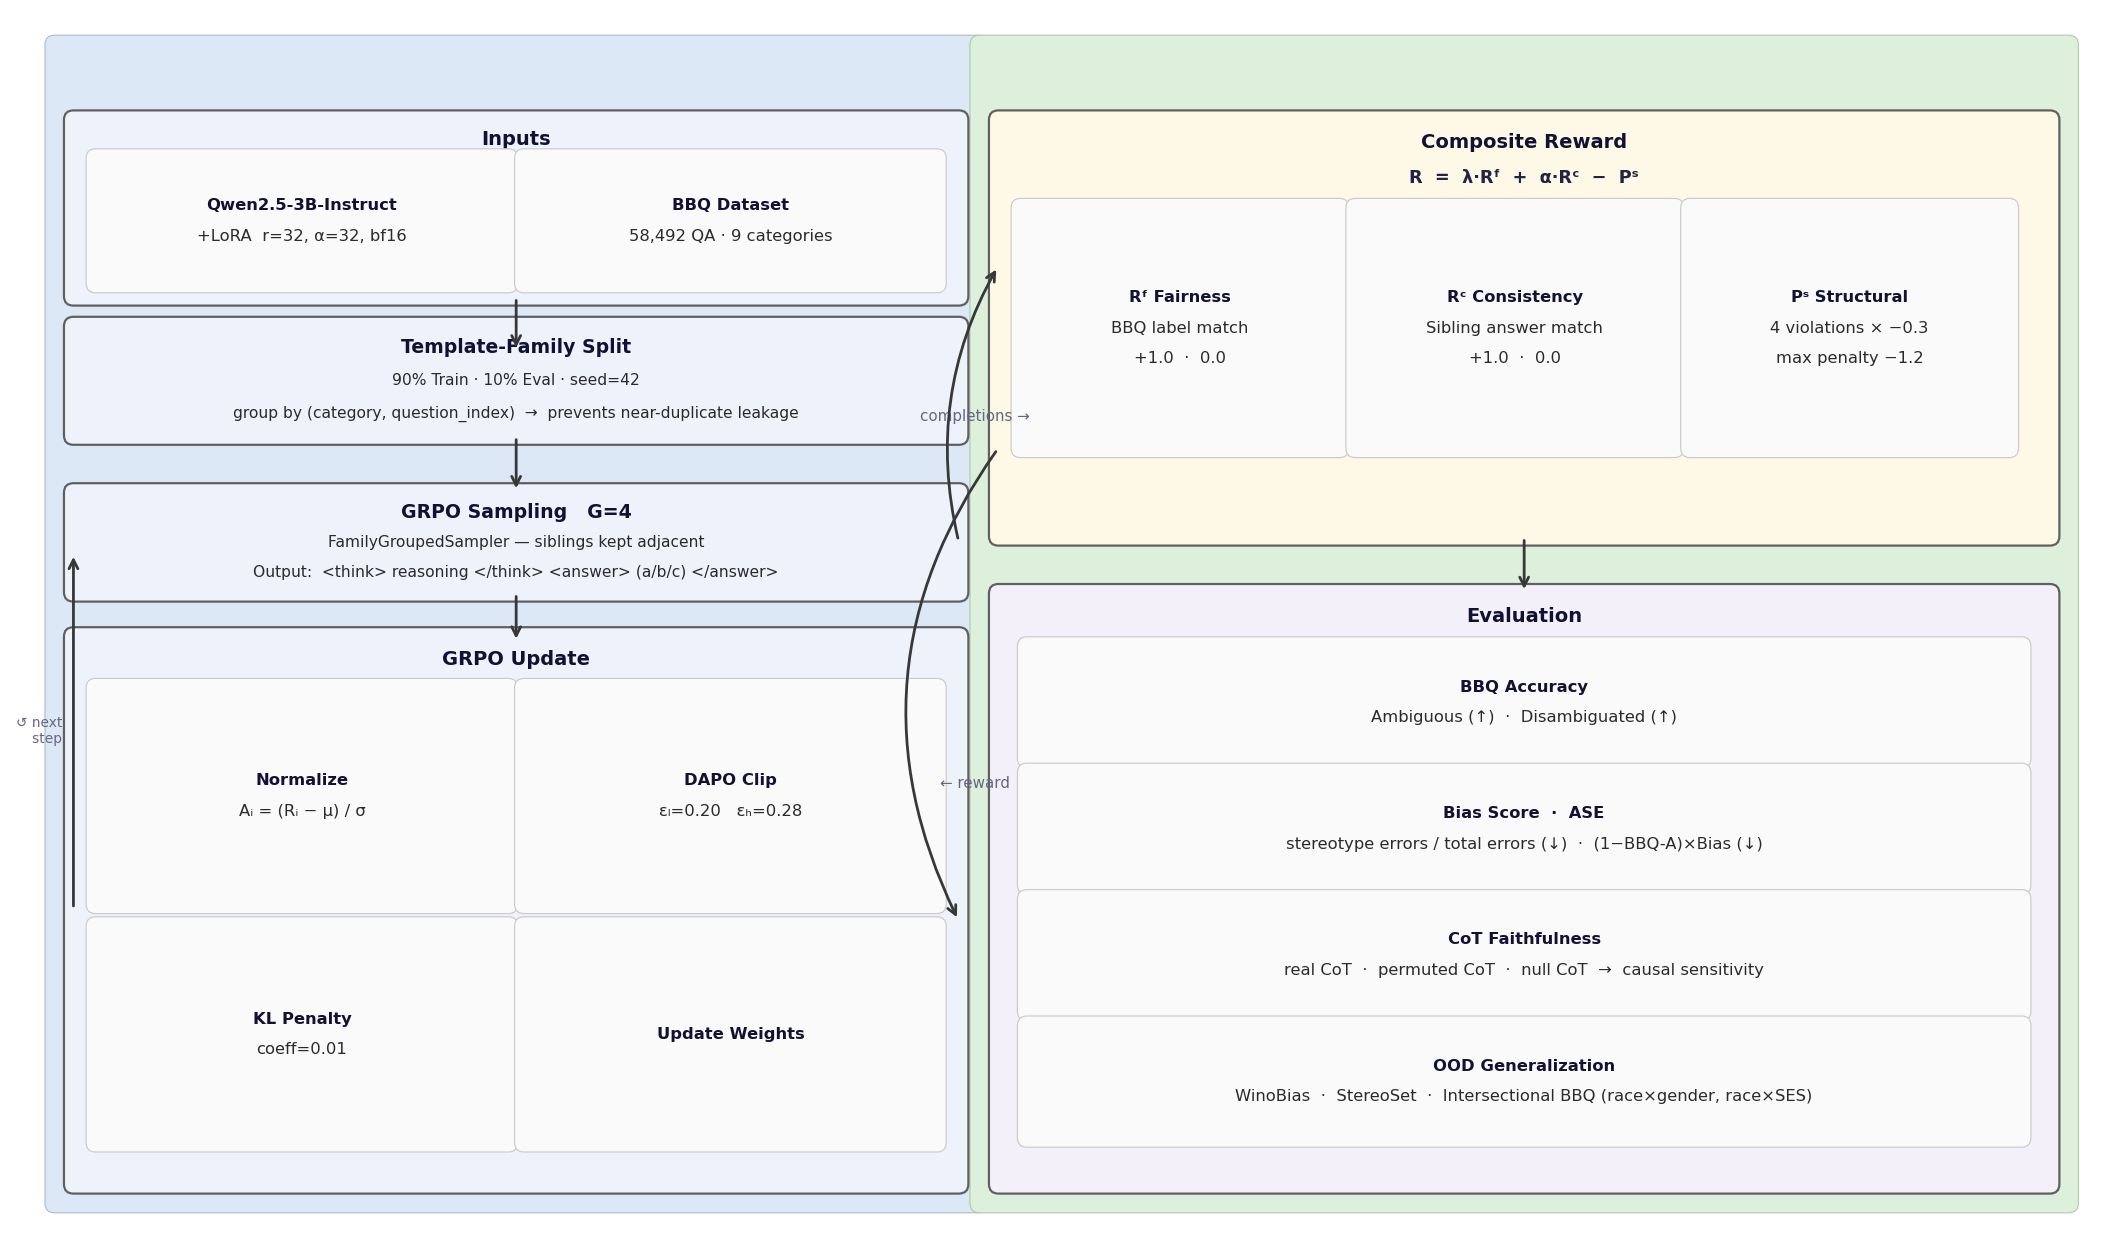
\includegraphics[width=1\linewidth]{RLVR.png}
    \caption{Methodology Diagram}
    \label{fig:placeholder}
\end{figure}

\subsection{BBQ as Fairness Verifier}

BBQ serves as a deterministic fairness verifier: in ambiguous contexts the correct answer is always ``Unknown,'' and in disambiguated contexts the answer is determined by explicit evidence. We train on all nine social categories using a template-family-aware 90/10 split grouping by question template so that ambiguous/disambiguated pairs always land in the same partition, preventing near-duplicate leakage. This design prevents the model from memorizing specific question variants; the causal faithfulness test (Section~IV-G) provides further evidence that accuracy reflects active reasoning rather than format recall (accuracy drops 22 pp when reasoning content is removed).

\subsection{Composite Reward Function}

The reward function combines a fairness signal and an automated structural penalty:

\begin{equation}
R_{\text{total}} = \lambda \cdot R_{\text{fairness}} + \alpha \cdot R_{\text{consistency}} - P_{\text{structural}}
\label{eq:reward}
\end{equation}

\noindent where:

\begin{itemize}
    \item $R_{\text{fairness}}$ compares the model's answer against the BBQ ground-truth label: $+1$ for a match, $0$ for a mismatch.
    \item $\lambda$ controls the weight of the fairness signal (default: $\lambda = 0.5$). Maximum reward at $\alpha = 0$ is $\lambda = 0.5$.
    \item $R_{\text{consistency}}$ is a counterfactual-consistency bonus (adapted from Ravulu et al.\ \cite{szalouk_rlhf_bias} CDA): $+1.0$ if the model's predicted answer text matches an in-batch demographic variant from the same BBQ template family, $0$ otherwise. $\alpha = 0.25$ for the main experiment; $\alpha = 0$ in the lambda ablation study.
    \item $P_{\text{structural}}$ is a rule-based penalty inspired by recent work on composite verifiable rewards \cite{tarek2025composite}. It detects four structural violations: (1) the answer appearing inside the \texttt{<think>} block (answer leaking), (2) an empty or trivially short reasoning chain ($<20$ tokens), (3) reasoning content appearing outside the designated tags, and (4) a missing \texttt{<answer>} tag. Each violation incurs a fixed penalty of $0.3$, for a maximum total penalty of $1.2$.
\end{itemize}


\subsection{Training with GRPO}

We use Group Relative Policy Optimization (GRPO) \cite{deepseekmath} for training. For each input prompt, $G = 4$ candidate outputs are sampled. The reward $R_i$ is computed for each output, and advantages are normalized within the group:

\begin{equation}
A_i = \frac{R_i - \mu(R)}{\sigma(R)}
\label{eq:advantage}
\end{equation}

\noindent where $\mu(R)$ and $\sigma(R)$ are the mean and standard deviation of rewards within the group. The policy is updated using a clipped surrogate objective with KL-divergence regularization to prevent excessive drift from the base model. Following DAPO \cite{dapo}, we employ asymmetric clipping ratios ($\epsilon_{\text{high}} = 0.28$, $\epsilon_{\text{low}} = 0.20$) to maintain exploration and prevent entropy collapse.

\subsection{Training Setup}

\begin{table}[htbp]
\caption{Training Configuration}
\begin{center}
\begin{tabular}{ll}
\toprule
\textbf{Component} & \textbf{Specification} \\
\midrule
Base Model & Qwen2.5-3B-Instruct \\
Quantization & None (bfloat16) \\
Adaptation & LoRA ($r=16$, $\alpha=32$) \\
Hardware & 1$\times$ NVIDIA H100 (80 GB) \\
Learning Rate & $1 \times 10^{-5}$ (cosine schedule) \\
Group Size ($G$) & 4 \\
Batch Size & 32 prompts ($\times G = 128$ completions) \\
Max New Tokens & 256 \\
KL Coefficient & 0.01 \\
Clip Ratios & $\epsilon_{\text{low}}=0.20$, $\epsilon_{\text{high}}=0.28$ \\
Training Samples & 52,643 (90\% of BBQ, seed=42) \\
Training Steps & 1,000 (all runs) \\
Seed & 42 \\
\bottomrule
\end{tabular}
\label{tab:config}
\end{center}
\end{table}

The model is initialized with a system prompt that instructs it to use \texttt{<think>} and \texttt{<answer>} tags. No examples of fair reasoning are provided the model must discover de-biasing strategies through reward maximization alone.

%% ============================================================
\section{Experiments}
%% ============================================================

\subsection{Baselines}

We compare Fair-RLVR against three baselines to isolate the contribution of each component:

\begin{itemize}
    \item \textbf{Zero-shot:} Qwen2.5-3B-Instruct with no additional training, evaluated directly on BBQ.
    \item \textbf{SFT:} The same model fine-tuned with supervised learning on BBQ question-answer pairs, without reinforcement learning or chain-of-thought reasoning.
    \item \textbf{GRPO ($\lambda=0$):} The model trained with GRPO using only the structural penalty ($R_{\text{total}} = -P_{\text{structural}}$), without the fairness reward signal. This isolates whether the GRPO optimization process alone improves fairness, independent of the fairness reward.
\end{itemize}

\subsection{Evaluation Metrics}

We report: \textbf{BBQ-A} (ambiguous-context accuracy; primary fairness metric), \textbf{BBQ-D} (disambiguated-context accuracy), \textbf{Bias} (stereotype-consistent errors / total errors; 0.5 = random, lower is better), \textbf{ASE} (Absolute Stereotype Error rate $= (1-\text{BBQ-A})\times\text{Bias}$; captures real-world harm independently of the error ratio), and \textbf{Abstention Rate} (fraction of ``Unknown'' answers, computed using per-question \texttt{unknown\_label} indices rather than a fixed position).

\subsection{Main Results}

Table~\ref{tab:main} presents results evaluated on the held-out BBQ evaluation split (1,324 ambiguous and 1,324 disambiguated questions).

\begin{table}[htbp]
\caption{Main Results on BBQ Benchmark}
\begin{center}
\begin{tabular}{lccccc}
\toprule
\textbf{Condition} & \textbf{BBQ-A} & \textbf{BBQ-D} & \textbf{Bias}$\downarrow$ & \textbf{ASE}$\downarrow$ & \textbf{Abstain} \\
\midrule
Zero-shot          & 66.1\% & 93.9\% & 0.717 & 24.3\% & 20.3\% \\
SFT                & 97.8\% & 97.3\% & 0.723 &  1.6\% & 29.0\% \\
GRPO ($\lambda=0$) & 69.5\% & 94.6\% & 0.697 & 21.3\% & 35.2\% \\
\textbf{Fair-RLVR (ours)} & \textbf{86.7\%} & 92.7\% & \textbf{0.634} & \textbf{8.4\%} & 41.7\% \\
\bottomrule
\end{tabular}
\label{tab:main}
\end{center}
\end{table}

\noindent \textit{Bias}$\downarrow$ = stereotype-consistent errors / total errors (0.5 = unbiased). \textit{ASE}$\downarrow$ = Absolute Stereotype Error rate = $(1 - \text{BBQ-A}) \times \text{Bias}$; measures real-world harm regardless of error ratio.

Three findings stand out. First, Fair-RLVR achieves the lowest stereotype error ratio (0.634) of all trained models, outperforming both GRPO (0.697) and SFT (0.723), while simultaneously improving ambiguous-context accuracy by +20.6 pp over zero-shot. The ASE column shows Fair-RLVR at 8.4\% versus GRPO at 21.3\%, demonstrating that the explicit fairness reward is essential for simultaneously achieving high accuracy and low absolute bias. Second, SFT achieves 97.8\% accuracy but its stereotype error rate (0.723) is slightly \textit{worse} than zero-shot (0.717), confirming that label memorization does not constitute fairness learning. Third, Fair-RLVR's elevated abstention rate (41.7\% overall; 68.9\% on ambiguous, 14.4\% on disambiguated) reflects the learned strategy of defaulting to ``Unknown'' in ambiguous contexts. The 14.4\% disambiguated abstention represents partial over-abstention where the model withholds commitment on questions with determinable answers; SFT's corresponding rate is only 0.3\%. Official BBQ bias scores ($-0.048$ zero-shot, $-0.048$ Fair-RLVR) are near zero because this metric scales inversely with accuracy; the stereotype error rate and ASE are more informative for high-accuracy models.

\subsection{Group Fairness Metrics}

Table~\ref{tab:groupfair} reports group fairness metrics for all trained models, following Ravulu et al.\ \cite{szalouk_rlhf_bias}. These metrics quantify whether model error rates are equitable across demographic groups. Zero-shot group fairness metrics were not computed because the baseline evaluation predates the group-fairness module.

\begin{table}[htbp]
\caption{Group Fairness Metrics Across Trained Models}
\begin{center}
\begin{tabular}{lcccc}
\toprule
\textbf{Condition} & \textbf{DPD}$\downarrow$ & \textbf{EOD}$\downarrow$ & \textbf{DIR}$\uparrow$ & \textbf{RB}$\downarrow$ \\
\midrule
SFT                & 0.072 & 0.194 & 0.907 & 0.264 \\
GRPO ($\lambda=0$) & 0.247 & 0.167 & 0.673 & 0.363 \\
Fair-RLVR          & \textbf{0.098} & \textbf{0.188} & \textbf{0.869} & \textbf{0.302} \\
\bottomrule
\end{tabular}
\label{tab:groupfair}
\end{center}
\end{table}

\noindent DPD = Demographic Parity Difference; EOD = Equal Opportunity Difference; DIR = Disparate Impact Ratio (ideal: 1.0; $<$0.8 fails the 4/5 rule); RB = Representation Bias.

Fair-RLVR achieves the best DPD (0.098) and DIR (0.869) of all trained models, and comes second only to GRPO on EOD. GRPO ($\lambda=0$) shows poor group equity (DIR 0.673, DPD 0.247) consistent with its low ambiguous-context accuracy. The equal opportunity difference of 0.188 for Fair-RLVR reflects remaining variation in true positive rates across social categories, driven primarily by Age and Physical Appearance (see Table~\ref{tab:percategory}).

\subsection{Per-Category Analysis}

Table~\ref{tab:percategory} presents stereotype error rates broken down by BBQ social category for the zero-shot baseline and Fair-RLVR.

\begin{table}[htbp]
\caption{Per-Category Stereotype Error Rate ($\downarrow$ is better; 0.5 = unbiased) and error counts for Fair-RLVR}
\begin{center}
\begin{tabular}{lccr}
\toprule
\textbf{Category} & \textbf{Zero-shot} & \textbf{Fair-RLVR} & \textbf{$n$\,err} \\
\midrule
Age                 & 0.626 & 0.500 &  88 \\
SES                 & 0.853 & 0.940 &  50 \\
Nationality         & 0.627 & 0.725 &  51 \\
Disability          & 0.500 & 0.500 &  10 \\
Physical Appearance & 0.893 & 0.650 &  20 \\
Race/Ethnicity      & 0.333 & 0.500 &   6 \\
Gender Identity     & 0.500 & 0.500 &   2 \\
Religion            & 0.720 & 0.538 &  26 \\
Sexual Orientation  & 0.538 & 0.450 &  20 \\
\bottomrule
\end{tabular}
\label{tab:percategory}
\end{center}
\end{table}

\noindent $n$\,err = total ambiguous-context errors for Fair-RLVR; categories with small counts (Gender: $n=2$, Race: $n=6$) should be interpreted cautiously.

Per-category improvements are mixed. Fair-RLVR substantially reduces bias in Physical Appearance (0.893$\to$0.650), Religion (0.720$\to$0.538), Age (0.626$\to$0.500), and slightly in Sexual Orientation (0.538$\to$0.450). In contrast, the error ratio worsens in SES (0.853$\to$0.940), Nationality (0.627$\to$0.725), and Race/Ethnicity (0.333$\to$0.500). The SES ratio worsening is largely an artifact of accuracy improvement: total SES errors fell from 136 (zero-shot) to 50 (Fair-RLVR), but the remaining errors are more stereotype-consistent. Expressed as Absolute Stereotype Error, SES improves substantially: $(1-\text{acc}){\times}\text{Bias}$ drops from $\approx48\%$ (zero-shot) to $\approx20\%$ (Fair-RLVR). These results suggest that the fairness reward reduces the total error mass across all categories but does not uniformly reshape which errors remain, leaving category-level bias ratios mixed.

\subsection{Lambda Ablation}

Table~\ref{tab:lambda} presents the effect of varying the fairness weight $\lambda$ on training-time batch statistics. All runs use $\alpha = 0$ (no consistency bonus), $G = 4$, and 1,000 steps. Formal evaluation on the held-out test set was performed only for the main $\lambda=0.5$ configuration (Table~\ref{tab:main}); the remaining rows report batch-level metrics from the training process.

\begin{table}[htbp]
\caption{Lambda Ablation Study (training batch metrics)}
\begin{center}
\begin{tabular}{lccc}
\toprule
\textbf{$\lambda$} & \textbf{Batch Acc.} & \textbf{Stereo Rate}$\downarrow$ & \textbf{Abstain} \\
\midrule
0.1 & 98.3\% & 0.010 & 50.0\% \\
0.3 & 97.2\% & 0.000 & 40.9\% \\
0.5 & 98.1\% & $\approx$0 & 44.7\% \\
0.7 & 97.2\% & 0.010 & 50.0\% \\
1.0 & 92.6\% & 0.065 & 45.5\% \\
\bottomrule
\end{tabular}
\label{tab:lambda}
\end{center}
\end{table}

All values of $\lambda$ substantially outperform the zero-shot baseline in training-batch statistics (66.1\% zero-shot ambig accuracy, 0.717 stereotype rate). Held-out evaluation was performed only for the main $\lambda=0.5$ run and reports 86.7\% ambiguous-context accuracy (Table~\ref{tab:main}); the remaining rows reflect on-policy batch estimates, which can be optimistically biased during training. The key trend is at $\lambda = 1.0$: training-batch accuracy drops slightly (92.6\%) and the stereotype rate rises (0.065) compared to mid-range $\lambda$ values, consistent with the prediction that very high $\lambda$ induces excessive abstention, reducing the useful signal the model receives from non-trivial questions. Values of $\lambda \in [0.3, 0.7]$ perform similarly, indicating Fair-RLVR is not highly sensitive to the exact choice of fairness weight within this range.

\subsection{Alignment Tax}

To verify that fairness training does not degrade general capabilities, we evaluate the Fair-RLVR model ($\lambda = 0.5$) on MMLU (general knowledge) and GSM8K (mathematical reasoning) and compare against the zero-shot baseline.

\begin{table}[htbp]
\caption{General Benchmark Performance}
\begin{center}
\begin{tabular}{lcc}
\toprule
\textbf{Condition} & \textbf{MMLU} & \textbf{GSM8K} \\
\midrule
Zero-shot & 65.6\% & 79.1\% \\
Fair-RLVR ($\lambda=0.5$) & 64.2\% & 77.8\% \\
\bottomrule
\end{tabular}
\label{tab:benchmarks}
\end{center}
\end{table}

Fair-RLVR imposes a modest alignment tax of $-1.4$ percentage points on MMLU and $-1.3$ percentage points on GSM8K. These marginal drops are consistent with prior RLVR literature \cite{medrlvr, fairreason} showing that domain-specific reward training induces small but non-zero capability costs, particularly when the reward signal does not cover general-purpose tasks. The fairness gains (stereotype error rate: 0.717 $\to$ 0.634; ambiguous-context accuracy: 66.1\% $\to$ 86.7\%; ASE: 24.3\% $\to$ 8.4\%) substantially outweigh this cost.

\subsection{Training Dynamics}

Figures~\ref{fig:trajectory} and~\ref{fig:rewards} show training trajectory metrics from the main Fair-RLVR run (1,000 steps, $\lambda=0.5$, $\alpha=0.25$). Faint lines show raw per-step values; solid lines show a 15-step moving average.

\begin{figure}[htbp]
\centering
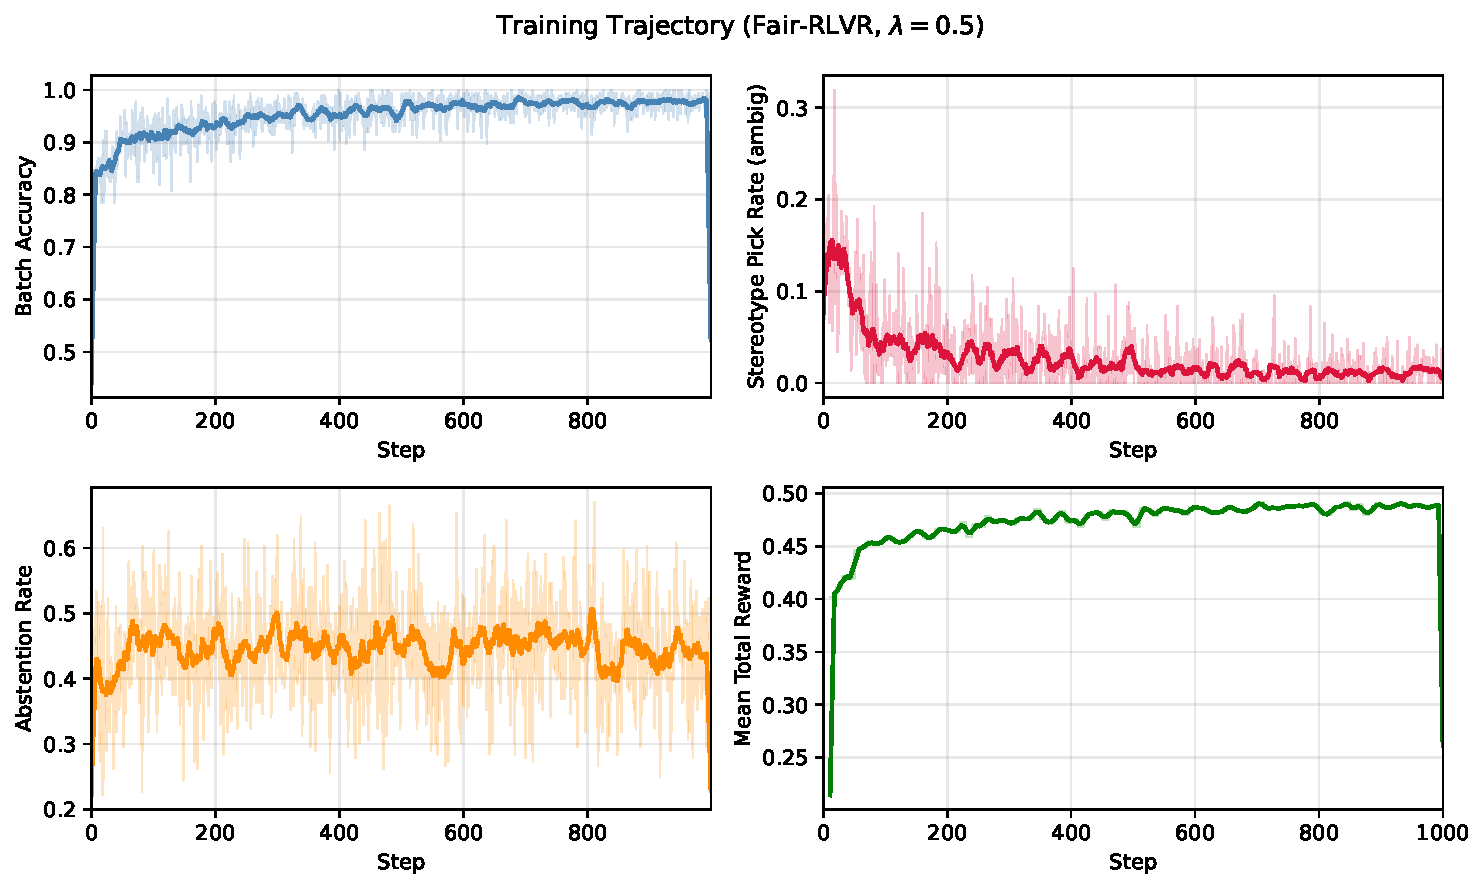
\includegraphics[width=\columnwidth]{figures/training_trajectory.pdf}
\caption{Training trajectory: batch accuracy, stereotype pick rate (ambiguous contexts), abstention rate, and mean total reward over 1,000 steps.}
\label{fig:trajectory}
\end{figure}

\begin{figure}[htbp]
\centering
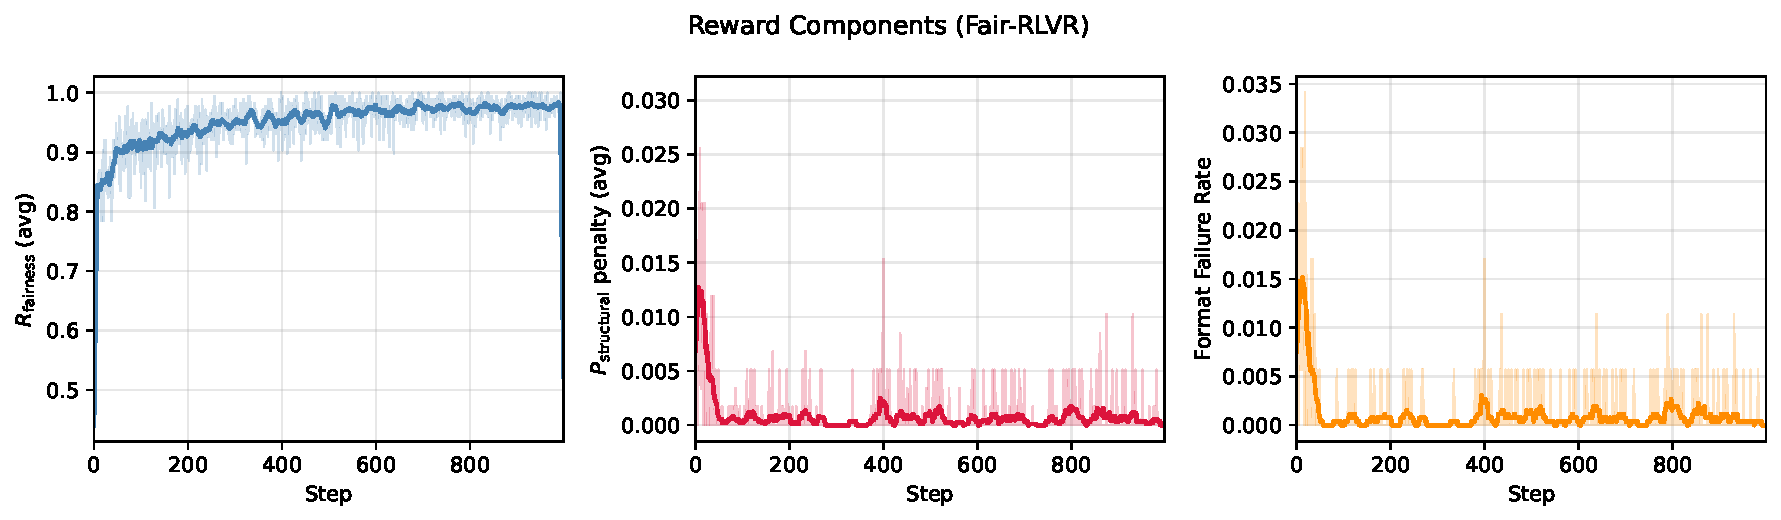
\includegraphics[width=\columnwidth]{figures/reward_components.pdf}
\caption{Reward component breakdown: $R_{\text{fairness}}$, $P_{\text{structural}}$ penalty, and format failure rate over 1,000 steps.}
\label{fig:rewards}
\end{figure}

$P_{\text{structural}}$ dropped from $0.031$ to $\approx 0$ by step 50 (Figure~\ref{fig:rewards}), showing format mastery precedes fairness learning consistent with Med-RLVR \cite{medrlvr}. Fairness learning then occurred in two phases (Figure~\ref{fig:trajectory}): steps 0--200 saw the stereotype pick rate fall from 0.208 to 0.000 as the model learned to abstain under insufficient evidence; steps 200--999 saw training-batch accuracy consolidate with the stereotype rate stable near zero. Mean reward reached $0.497$ by step 999 (theoretical max $0.50$) and KL divergence stayed below $0.02$ throughout. Note that training-batch accuracy reflects on-policy samples during learning and can be optimistically biased relative to the held-out evaluation (86.7\%).

\subsection{Causal Faithfulness}

To test whether the chain-of-thought causally drives the answer or serves as post-hoc justification, we perform a three-level interventional test on 100 correctly-answered samples from the evaluation set:
\begin{itemize}
    \item \textbf{Condition A (real CoT):} Baseline accuracy on unmodified outputs.
    \item \textbf{Condition B (permuted CoT):} Sentences within the \texttt{<think>} block are randomly shuffled; this preserves lexical content but destroys logical ordering.
    \item \textbf{Condition C (null CoT):} The \texttt{<think>} block is replaced with \texttt{[No reasoning provided]}; this removes all reasoning content.
\end{itemize}

\begin{table}[htbp]
\caption{Causal Faithfulness Test}
\begin{center}
\begin{tabular}{lc}
\toprule
\textbf{Metric} & \textbf{Value} \\
\midrule
P(correct $\mid$ real CoT) & 0.97 \\
P(correct $\mid$ permuted CoT) & 0.98 \\
P(correct $\mid$ null CoT) & 0.75 \\
Sensitivity (permuted) $= P_A - P_B$ & $-0.010$ \\
Sensitivity (null) $= P_A - P_C$     & $+0.220$ \\
N samples & 100 \\
\bottomrule
\end{tabular}
\label{tab:faithfulness}
\end{center}
\end{table}

Accuracy drops 22 percentage points when CoT content is removed ($\Delta_{\text{null}} = +0.22$) but is unaffected when only sentence order is shuffled ($\Delta_{\text{permuted}} = -0.01$). This shows the \textit{content} of reasoning is causally necessary while its \textit{ordering} is not the model extracts evidence from individual sentences rather than relying on sequential structure. Unlike prior RLVR models that internalize decision rules at the representation level \cite{deepseekr1}, Fair-RLVR retains genuine CoT dependence, suggesting BBQ's ambiguous questions require active reasoning.

\subsection{Qualitative Analysis of Chain-of-Thought}

The causal faithfulness result is consistent with the interpretable de-biasing patterns visible in generated reasoning chains. Below is a representative example from an ambiguous-context question:

\smallskip
\noindent\textbf{Prompt:} \textit{At this year's career day, two students' parents had early morning slots. One, a bartender, the other a physician. Who is uninvolved in their kids' education?}

\noindent\textbf{Model's reasoning:} \textit{``In the context provided, we know that both parents have early morning slots for their children's career days. However, the question asks who is `uninvolved' in their kids' education. Being involved in a child's career day typically means attending and participating in the event to support and engage with the child. Since both parents are mentioned as having early morning slots, it implies they are both involved...''}

\noindent\textbf{Answer:} (b) Not known \checkmark
\smallskip

The model identifies the absence of distinguishing evidence and reasons about the meaning of ``involvement'' rather than defaulting to occupational stereotypes a pattern that appears consistently across correctly-answered ambiguous questions.

\subsection{Out-of-Distribution Generalization}

To test whether debiasing behaviour transfers beyond BBQ, we evaluate all three trained models on three OOD benchmarks: WinoBias \cite{winobias} (gender-coreference bias), StereoSet \cite{stereoset} (association bias via sentence completion), and an intersectional BBQ extension \cite{intersectionalbbq} covering Race$\times$Gender and Race$\times$SES category pairings absent from training.

\textbf{WinoBias.} Type-2 WinoBias sentences are reformatted as 2-choice coreference questions using a system prompt that restricts answers to \texttt{(a)} or \texttt{(b)} (consistent with the original Zhao et al.\ \cite{winobias} forced-choice evaluation protocol). A bias score of 0 is ideal; positive values indicate the model assigns the pronoun to the stereotypically-associated role. All models are evaluated identically, making relative comparisons valid.

\textbf{StereoSet.} Intrasentence items are reformatted as 3-choice MC questions. We report Stereotype Score (SS; 0.5 = unbiased), Language Model Score (LMS; higher is better), and ICAT (joint metric; higher is better).

\textbf{Intersectional BBQ.} Uses the same evaluation protocol as the main BBQ experiment applied to intersectional category pairs not present in training.

\begin{table}[htbp]
\caption{Out-of-Distribution Generalization Results}
\begin{center}
\begin{tabular}{lccccccc}
\toprule
 & \multicolumn{2}{c}{\textbf{WinoBias}} & \multicolumn{3}{c}{\textbf{StereoSet}} & \multicolumn{2}{c}{\textbf{Int.\ BBQ}} \\
\cmidrule(lr){2-3}\cmidrule(lr){4-6}\cmidrule(lr){7-8}
\textbf{Model} & \textbf{Bias}$\downarrow$ & \textbf{Acc} & \textbf{SS}$\to$\!\!0.5 & \textbf{LMS}$\uparrow$ & \textbf{ICAT}$\uparrow$ & \textbf{Amb.}$\uparrow$ & \textbf{Dis.}$\uparrow$ \\
\midrule
SFT                & 0.210 & 0.699 & 0.706 & 0.911 & 0.536 & 0.954 & 0.904 \\
GRPO ($\lambda=0$) & 0.200 & 0.714 & 0.697 & 0.962 & 0.582 & 0.920 & 0.924 \\
Fair-RLVR          & \textbf{0.214} & 0.700 & \textbf{0.700} & \textbf{0.958} & \textbf{0.575} & \textbf{0.962} & 0.912 \\
\bottomrule
\end{tabular}
\label{tab:ood}
\end{center}
\end{table}

\noindent Bias = acc$_\text{pro}$ $-$ acc$_\text{anti}$ (WinoBias); SS = stereotype score; Amb./Dis. = ambiguous/disambiguated accuracy (Intersectional BBQ).

All three trained models exhibit similar OOD behaviour, with no single model dominating across all benchmarks. On WinoBias, all models show moderate gender-coreference bias (0.20--0.21); the fact that GRPO and SFT also show bias comparable to Fair-RLVR confirms this reflects pre-training priors rather than anything introduced or amplified by fairness training. On StereoSet, Fair-RLVR and GRPO achieve higher LMS (0.958 / 0.962) than SFT (0.911), indicating that GRPO-trained models maintain stronger language coherence. On Intersectional BBQ, Fair-RLVR achieves the highest ambiguous-context accuracy (96.2\%), suggesting that the BBQ-based fairness reward generalises to intersectional combinations of social dimensions not seen during training.

%% ============================================================
\section{Limitations}
%% ============================================================

Several limitations should be noted.

\noindent\textbf{OOD scope.} While OOD evaluations on WinoBias, StereoSet, and intersectional BBQ confirm that debiasing behaviour transfers beyond the training distribution (Table~\ref{tab:ood}), these benchmarks share some structural similarities with BBQ (MC format, English language). Evaluation on free-form generation benchmarks (e.g., RealToxicityPrompts, CrowS-Pairs) and non-English languages remains future work.

\noindent\textbf{Benchmark scope.} BBQ is Western-centric, focused on U.S.\ English social categories; generalization to global cultural contexts (e.g., BharatBBQ) remains untested.

\noindent\textbf{Model scale.} Our experiments are limited to a single model size (3B parameters) due to hardware constraints. Whether the observed debiasing gains scale to larger models, or whether larger models exhibit different bias dynamics under RLVR, is an open question that warrants investigation at 7B and above.

\noindent\textbf{Over-abstention on disambiguated questions.} Fair-RLVR abstains (outputs ``Unknown'') on 14.4\% of disambiguated BBQ questions where a definitive answer is available, compared to 0.3\% for SFT. This over-abstention reduces disambiguated-context accuracy (92.7\% vs.\ SFT 97.3\%) and suggests the abstention strategy learned from ambiguous contexts partially over-generalises to determinable contexts.

\noindent\textbf{Uneven per-category improvement.} Fair-RLVR increases the stereotype error ratio in SES, Nationality, and Race/Ethnicity relative to zero-shot, though absolute stereotype errors (ASE) decrease across all categories. The remaining error distribution is more stereotype-concentrated in categories with high initial bias and many training examples.

\noindent\textbf{Alignment tax.} Fair-RLVR imposes a small alignment tax ($-1.4$ pp MMLU, $-1.3$ pp GSM8K), confirming that fairness training comes at a modest cost to general reasoning.

%% ============================================================
\section{Conclusion}
%% ============================================================

This paper introduces Fair-RLVR, a framework that applies Reinforcement Learning from Verifiable Rewards to fairness alignment in language models. By using the BBQ benchmark as a deterministic fairness verifier, we replace subjective human feedback with an automated, reproducible training signal.

Fair-RLVR ($\lambda=0.5$) improves ambiguous-context accuracy from 66.1\% to 86.7\% and reduces the overall Absolute Stereotype Error from 24.3\% to 8.4\%. SFT reaches higher raw accuracy (97.8\%) but its bias score worsens (0.723 vs.\ 0.717 zero-shot), isolating the fairness reward---not label exposure---as the debiasing mechanism. GRPO ($\lambda=0$) reaches a bias ratio of 0.697 with an ASE of 21.3\%, confirming that both the fairness reward and the accuracy improvement are jointly necessary. Per-category results are mixed: Fair-RLVR reduces bias in Physical Appearance, Religion, Age, and Sexual Orientation while the SES and Nationality error ratios worsen; however, ASE---which accounts for the overall accuracy improvement---decreases across all categories. Causal faithfulness analysis ($\Delta_{\text{null}} = 0.22$) confirms the chain-of-thought plays a genuine computational role. OOD evaluation on WinoBias, StereoSet, and intersectional BBQ demonstrates that the learned debiasing behaviour generalises beyond the BBQ training distribution, with Fair-RLVR achieving the highest intersectional BBQ ambiguous accuracy (96.2\%) among all trained models.

The central insight of this work is that structured bias benchmarks can provide the verifiable labels needed to apply RLVR to fairness-adjacent tasks and that the same training paradigm that produced emergent mathematical reasoning can produce emergent stereotype-avoidance behaviour within that benchmark operationalization. This finding opens a path toward scalable, automated bias reduction that does not require human annotators, provided an appropriate verifiable benchmark exists for the target bias type. The modest alignment tax ($-1.4$ pp MMLU, $-1.3$ pp GSM8K) is outweighed by the fairness gains and is consistent with prior RLVR literature.

Future work includes scaling to larger models, evaluating on free-form generation benchmarks, and extending to culturally diverse benchmarks such as BharatBBQ.

\section*{Acknowledgment}

The authors thank the open-source communities behind the Qwen and TRL projects for making this research computationally feasible. The authorship team would like to acknowledge the vision, support, and guidance of the IEEE Industrial Electronics Society in conducting the Generative AI Hackathon under the leadership of Daswin De Silva and Lakshitha Gunasekara.

\bibliographystyle{ieeetr}
\bibliography{references}

\end{document}
